\documentclass[12pt,a4paper]{report}
\usepackage[utf8]{inputenc}
\usepackage{amsmath}
\usepackage{amsfonts}
\usepackage{amssymb}
\usepackage{amsthm}
\usepackage{hyperref}

\usepackage{multicol}
\usepackage{fancyhdr}
\usepackage[inline]{enumitem}
\usepackage{tikz}
\usepackage{tikz-cd}
\usetikzlibrary{calc}
\usetikzlibrary{shapes.geometric}
\usetikzlibrary{positioning}
\usepackage[margin=0.5in]{geometry}
\usepackage{xcolor}

\hypersetup{
    colorlinks=true,
    linkcolor=blue,
    filecolor=magenta,      
    urlcolor=cyan,
    pdftitle={Tensors},
    pdfpagemode=FullScreen,
    }

%\urlstyle{same}

\newcommand{\CLASSNAME}{Math 5050 -- Special Topics: Manifolds}
\newcommand{\STUDENTNAME}{Paul Carmody}
\newcommand{\ASSIGNMENT}{Section 9: Submanifolds }
\newcommand{\DUEDATE}{June 11, 2025}
\newcommand{\PROFESSOR}{Professor Berchenko-Kogan}
\newcommand{\SEMESTER}{Fall 2025}
\newcommand{\SCHEDULE}{TBD}
\newcommand{\ROOM}{Remote}

\newcommand{\MMN}{M_{m\times n}}
\newcommand{\FF}{\mathcal{F}}

\pagestyle{fancy}
\fancyhf{}
\chead{ \fancyplain{}{\CLASSNAME} }
%\chead{ \fancyplain{}{\STUDENTNAME} }
\rhead{\thepage}
\newcommand{\LET}{\text{Let }}
%\newcommand{\IF}{\text{if }}
\newcommand{\AND}{\text{ and }}
\newcommand{\OR}{\text{ or }}
\newcommand{\FORSOME}{\text{ for some }}
\newcommand{\FORALL}{\text{ for all }}
\newcommand{\WHERE}{\text{ where }}
\newcommand{\WTS}{\text{ WTS }}
\newcommand{\WLOG}{\text{ WLOG }}
\newcommand{\BS}{\backslash}
\newcommand{\DEFINE}[1]{\textbf{\emph{#1}}}
\newcommand{\IF}{$(\Rightarrow)$}
\newcommand{\ONLYIF}{$(\Leftarrow)$}
\newcommand{\ITH}{\textsuperscript{th} }
\newcommand{\FST}{\textsuperscript{st} }
\newcommand{\SND}{\textsuperscript{nd} }
\newcommand{\TRD}{\textsuperscript{rd} }
\newcommand{\INV}{\textsuperscript{-1} }

\newcommand{\XXX}{\mathfrak{X}}
\newcommand{\MMM}{\mathfrak{M}}
%\newcommand{\????}{\textfrak{A}}
%\newcommand{\????}{\textgoth{A}}
%\newcommand{\????}{\textswab{A}}

\DeclareMathOperator{\DER}{Der}
\DeclareMathOperator{\SGN}{sgn}

%%%%%%%
% derivatives
%%%%%%%

\newcommand{\PART}[2]{\frac{\partial #1}{\partial #2}}
\newcommand{\SPART}[2]{\frac{\partial^2 #1}{\partial #2^2}}
\newcommand{\DERIV}[2]{\frac{d #1}{d #2}}
\newcommand{\LAPLACIAN}[1]{\frac{\partial^2 #1}{\partial x^2} + \frac{\partial^2 #1}{\partial y^2}}

%%%%%%%
% sum, product, union, intersections
%%%%%%%

\newcommand{\SUM}[2]{\underset{#1}{\overset{#2}{\sum}}}
\newcommand{\PROD}[2]{\underset{#1}{\overset{#2}{\prod}}}
\newcommand{\UNION}[2]{\underset{#1}{\overset{#2}{\bigcup}}}
\newcommand{\INTERSECT}[2]{\underset{#1}{\overset{#2}{\bigcap}}}
\newcommand{\FSUM}{\SUM{n=-\infty}{\infty}}
       

%%%%%%%
% supremum and infimum
%%%%%%%

\newcommand{\SUP}[1]{\underset{#1}\sup \,}
\newcommand{\INF}[1]{\underset{#1}\inf \,}
\newcommand{\MAX}[1]{\underset{#1}\max \,}
\newcommand{\MIN}[1]{\underset{#1}\min \,}

%%%%%%%
% infinite sums, limits
%%%%%%%

\newcommand{\SUMK}{\SUM{k=1}{\infty}}
\newcommand{\SUMN}{\SUM{n=1}{\infty}}
\newcommand{\SUMKZ}{\SUM{k=0}{\infty}}
\newcommand{\LIM}[1]{\underset{#1}\lim\,}
\newcommand{\IWOB}[1]{\LIM{#1 \to \infty}}
\newcommand{\LIMK}{\IWOB{k}}
\newcommand{\LIMN}{\IWOB{n}}
\newcommand{\LIMX}{\IWOB{x}}
\newcommand{\NIWOB}{\LIM{n \to \infty}}
\newcommand{\LIMSUPK}{\underset{k\to\infty}\limsup \,}
\newcommand{\LIMSUPN}{\underset{n\to\infty}\limsup \,}
\newcommand{\LIMINFK}{\underset{k\to\infty}\liminf \,}
\newcommand{\LIMINFN}{\underset{n\to\infty}\liminf \,}
\newcommand{\ROOTRULE}[1]{\LIMSUPK \BARS{#1}^{1/k}}

\newcommand{\CUPK}{\bigcup_{k=1}^{\infty}}
\newcommand{\CAPK}{\bigcap_{k=1}^{\infty}}
\newcommand{\CUPN}{\bigcup_{n=1}^{\infty}}
\newcommand{\CAPN}{\bigcap_{n=1}^{\infty}}

%%%%%%%
% number systems (real, rational, etc.)
%%%%%%%

\newcommand{\REALS}{\mathbb{R}}
\newcommand{\RATIONALS}{\mathbb{Q}}
\newcommand{\IRRATIONALS}{\REALS \backslash \RATIONALS}
\newcommand{\INTEGERS}{\mathbb{Z}}
\newcommand{\NUMBERS}{\mathbb{N}}
\newcommand{\COMPLEX}{\mathbb{C}}
\newcommand{\DISC}{\mathbb{D}}
\newcommand{\HPLANE}{\mathbb{H}}

\newcommand{\R}{\mathbb{R}}
\newcommand{\Q}{\mathbb{Q}}
\newcommand{\Z}{\mathbb{Z}}
\newcommand{\N}{\mathbb{N}}
\newcommand{\C}{\mathbb{C}}
\newcommand{\T}{\mathbb{T}}
\newcommand{\COUNTABLE}{\aleph_0}
\newcommand{\UNCOUNTABLE}{\aleph_1}


%%%%%%%
% Arithmetic/Algebraic operators
%%%%%%%


\DeclareMathOperator{\MOD}{mod}
%\newcommand{\MOD}[1]{\mod #1}
\newcommand{\BAR}[1]{\overline{#1}}
\newcommand{\LCM}{\text{ lcm}}
\newcommand{\ZMOD}[1]{\Z/#1\Z}
\DeclareMathOperator{\VAR}{Var}
%%%%%%%
% complex operators
%%%%%%%

\DeclareMathOperator{\RR}{Re}
%\newcommand{\RE}{\text{Re}}
\DeclareMathOperator{\IM}{Im}
%\newcommand{\IM}{\text{Im}}
\newcommand{\CONJ}[1]{\overline{#1}}
\DeclareMathOperator{\LOG}{Log}
%\newcommand{\LOG}{\text{ Log }}
\newcommand{\RES}[2]{\underset{#1}{\text{res}} #2}

%%%%%%%
% Group operators
%%%%%%%

\newcommand{\AUT}{\text{Aut}\,}
\newcommand{\KER}{\text{ker}\,}
\newcommand{\END}{\text{End}}
\newcommand{\HOM}{\text{Hom}}
\newcommand{\CYCLE}[1]{(\begin{array}{cccccccccc}
		#1
	\end{array})}
\newcommand{\SUBGROUP}{\underset{\text{group}}\subseteq}	
%\newcommand{\SUBGROUP}{\subseteq_g}
\newcommand{\SUBRING}{\underset{\text{ring}}\subseteq}
\newcommand{\SUBMOD}{\underset{\text{mod}}\subseteq}
\newcommand{\SUBFIELD}{\underset{\text{field}}\subseteq}
\newcommand{\ISO}{\underset{\text{iso}}\longrightarrow}
\newcommand{\HOMO}{\underset{\text{homo}}\longrightarrow}

%%%%%%%
% grouping (parenthesis, absolute value, square, multi-level brackets).
%%%%%%%

\newcommand{\PAREN}[1]{\left (\, #1 \,\right )}
\newcommand{\BRACKET}[1]{\left \{\, #1 \,\right \}}
\newcommand{\SQBRACKET}[1]{\left [\, #1 \,\right ]}
\newcommand{\ABRACKET}[1]{\left \langle\, #1 \,\right \rangle}
\newcommand{\BARS}[1]{\left |\, #1 \,\right |}
\newcommand{\DBARS}[1]{\left \| \, #1 \,\right \|}
\newcommand{\LBRACKET}[1]{\left \{ #1 \right .} 
\newcommand{\RBRACKET}[1]{\left . #1 \right \]}
\newcommand{\RBAR}[1]{\left . #1 \, \right |}
\newcommand{\LBAR}[1]{\left | \, #1 \right .}
\newcommand{\BLBRACKET}[2]{\BRACKET{\RBAR{#1}#2}}
\newcommand{\GEN}[1]{\ABRACKET{#1}}
\newcommand{\BINDEF}[2]{\LBRACKET{\begin{array}{ll}
     #1\\
     #2
\end{array}}}

%%%%%%%
% Fourier Analysis
%%%%%%%

\newcommand{\ONEOTWOPI}{\frac{1}{2\pi}}
\newcommand{\FHAT}{\hat{f}(n)}
\newcommand{\FINT}{\int_{-\pi}^\pi}
\newcommand{\FINTWO}{\int_{0}^{2\pi}}
\newcommand{\FSUMN}[1]{\SUM{n=-#1}{#1}}
%\newcommand{\FSUM}{\SUMN{\infty}}
\newcommand{\EIN}[1]{e^{in#1}}
\newcommand{\NEIN}[1]{e^{-in#1}}
\newcommand{\INTALL}{\int_{-\infty}^{\infty}}
\newcommand{\FTINT}[1]{\INTALL #1 e^{2\pi inx\xi} dx}
\newcommand{\GAUSS}{e^{-\pi x^2}}

%%%%%%%
% formatting 
%%%%%%%

\newcommand{\LEFTBOLD}[1]{\noindent\textbf{#1}}
\newcommand{\SEQ}[1]{\{#1\,\}}
\newcommand{\WIP}{\footnote{work in progress}}
\newcommand{\QED}{\hfill\square}
\newcommand{\ts}{\textsuperscript}
\newcommand{\HLINE}{\noindent\rule{7in}{1pt}\\}

%%%%%%%
% Mathematical note taking (definitions, theorems, etc.)
%%%%%%%

\newcommand{\REM}{\noindent\textbf{\\Remark: }}
\newcommand{\DEF}{\noindent\textbf{\\Definition: }}
\newcommand{\THE}{\noindent\textbf{\\Theorem: }}
\newcommand{\COR}{\noindent\textbf{\\Corollary: }}
\newcommand{\LEM}{\noindent\textbf{\\Lemma: }}
\newcommand{\PROP}{\noindent\textbf{\\Proposition: }}
\newcommand{\PROOF}{\noindent\textbf{\\Proof: }}
\newcommand{\EXP}{\noindent\textbf{\\Example: }}
\newcommand{\TRICKS}{\noindent\textbf{\\Tricks: }}


%%%%%%%
% text highlighting
%%%%%%%

\newcommand{\B}[1]{\textbf{#1}}
\newcommand{\CAL}[1]{\mathcal{#1}}
\newcommand{\UL}[1]{\underline{#1}}

%%%%%%
% Linear Algebra
%%%%%%

\newcommand{\COLVECTOR}[1]{\PAREN{\begin{array}{c}
#1
\end{array} }}
\newcommand{\TWOXTWO}[4]{\PAREN{ \begin{array}{c c} #1&#2 \\ #3 & #4 \end{array} }}
\newcommand{\DTWOXTWO}[4]{\BARS{ \begin{array}{c c} #1&#2 \\ #3 & #4 \end{array} }}
\newcommand{\THREEXTHREE}[9]{\PAREN{ \begin{array}{c c c} #1&#2&#3 \\ #4 & #5 & #6 \\ #7 & #8 & #9 \end{array} }}
\newcommand{\DTHREEXTHREE}[9]{\BARS{ \begin{array}{c c c} #1&#2&#3 \\ #4 & #5 & #6 \\ #7 & #8 & #9 \end{array} }}
\newcommand{\NXN}{\PAREN{ \begin{array}{c c c c} 
			a_{11} & a_{12} & \cdots & a_{1n} \\
			a_{21} & a_{22} & \cdots & a_{2n} \\
			\vdots & \vdots & \ddots & a_{1n} \\
			a_{n1} & a_{n2} & \cdots & a_{nn} \\
		\end{array} }}
\newcommand{\SLR}{SL_2(\R)}
\newcommand{\GLR}{GL_2(\R)}
\DeclareMathOperator{\TR}{tr}
\DeclareMathOperator{\BIL}{Bil}
\DeclareMathOperator{\SPAN}{span}

%%%%%%%
%  White space
%%%%%%%

\newcommand{\BOXIT}[1]{\noindent\fbox{\parbox{\textwidth}{#1}}}


\newtheorem{theorem}{Theorem}[section]
\newtheorem{corollary}{Corollary}[theorem]
\newtheorem{lemma}[theorem]{Lemma}

\theoremstyle{definition}
\newtheorem{definition}[theorem]{Definition}
\newtheorem{prop}[theorem]{Proposition}

\theoremstyle{remark}
\newtheorem{remark}[theorem]{Remark}
\newtheorem{example}[theorem]{Example}
%\newtheorem*{proof}[theorem]{Proof}



\newcommand{\RED}[1]{\textcolor{red}{#1}}
\newcommand{\BLUE}[1]{\textcolor{blue}{#1}}

\begin{document}

\begin{center}
	\Large{\CLASSNAME -- \SEMESTER} \\
	\large{ w/\PROFESSOR}
\end{center}
\begin{center}
	\STUDENTNAME \\
	\ASSIGNMENT -- \DUEDATE\\
\end{center} 


\noindent \textbf{\\\large{Problems}}

\begin{enumerate}[label=9.\arabic*.]

\item \textbf{Regular values}

Define $f:\R^2\to \R$ by
\begin{align*}
	f(x,y) = x^3-6xy+y^2.
\end{align*}Find all values $c \in \R$ for which the level $f^{-1}(c)$ is a regular submanifold of $\R^2$.

\BLUE{Stated another way: find all of the $p \in \R^2$ such that $f(p)=c$ and $p$ is regular (i.e., not a critical point).  Regular points are points that have a non-zero Jacobian.  Thus,
\begin{align*}
	J(f) &= \PAREN{\PART{f}{x},\PART{f}{y}} = \PAREN{3x^2-6y, -6x+2y} \\
	J(f) &= 0 \\
	x^2-3y &= 0 \AND y= 3x \\
	3x &= \frac{x^2}{3} \\
	\frac{x^2}{3} -3x &= 0 \implies x=0,6 \\
	y &= 0, 18
\end{align*}thus, these points $(0,0), (6,18)$ are the critical points which will NOT be in a smooth manifold (non-regular points).  Therefore, the values of $c$ are which do not work are
\begin{align*}
	f(0,0) &= 0 \\
	f(6,18) &= 6^3-6(6)(18)+18^2 = -108 \\
\end{align*}Thus $c \in \R \backslash \{0, -108\}$
}

\item \textbf{Solution set of one equation.}

Let $x,y,z,w$ be the standard coordinates on $\R^4$.  Is the solution set of $x^5+y^5+z^5+w^5=1$ in $\R^4$ a smooth manifold?  Explain why or why not.  (Assume that the subset is given the subspace topology).

\BLUE{The Jacobian is essentially the gradient.
\begin{align*}
	\LET f(x,y,z,w) &= x^5+y^5+z^5+w^5-1 \\
	\nabla f(x,y,z,w) &= (5x^4, 5y^4, 5z^4, 5w^4)\\
	\nabla f &= 0 \implies (0,0,0,0)
\end{align*}but $(0,0,0,0)$ is not a solution of $f$.  Therefore the solution space is smooth.
}

\item \textbf{Solution set of two equations.}

Is the solution set of the system of equations 
\begin{align*}
	x^3+y^3+z^3=1,\, z=xy
\end{align*}in $\R^3$ a smooth manifold?  Prove your answer.

\BLUE{Let $F: \R^3 \to \R^2$ and $F(x,y,z) = (x^3+y^3+z^3-1,\, z-xy)$.  Then
\begin{align*}
	J(F) &= \SQBRACKET{\begin{array}{ccc}
		3x^2 & 3y^2 & 3z^2 \\
		-y & -x & 1
	\end{array}
	}
\end{align*}are these two linearly independent?  Is there a $\lambda$ such that 
\begin{align*}
	3x^2 &= \lambda(-y), \, 3y^2 = \lambda(-x), \, 3z^2 = \lambda \\
	-3x^2/y &= -3y^2/x \to x^3 = y^3 \to x=y\\
	3x^2 &= \lambda(-x) \to \lambda = -3x \\
	-3x &= 3z^2 \to -x=z^2 \AND z=xy=x^2 \implies x = 0, 1
\end{align*}Thus, $(0,0,0)$ is a critical point but doesn't exist in the range of $F_x$ therefore the solution set is a submanifold.
}

\item \textbf{Regular submanifolds}

Suppose that a subset $S$ of $\R^2$ that the property that locally on $S$ one of the coordinates is $C^\infty$ function of the other coordinate.  Show that $S$ is a regular submanifold of $\R^2$. (Note that the unit circle defined by $x^2+y^2=1$ has this property at every point of the circle, there is a neighborhood in which $y$ is a $C^\infty$ function of $x$ or $x$ is a $C^\infty$ function of $y$.)

\item \textbf{Graph of a smooth function}

Show that the graph $\Gamma(f)$ of a smooth function $f: \R^2\to \R$.
\begin{align*}
	\Gamma(f) &= \BRACKET{\PAREN{x,y,f(x,y)} \in \R^3}
\end{align*}is a regular submanifold of $\R^3$.

\BLUE{Redefine $\Gamma$ as \begin{align*}
	\Gamma(x,y,z) &= z-f(x,y) = 0\\
	J(\Gamma) &= \SQBRACKET{\begin{array}{ccc}
		\PART{\Gamma}{x} & \PART{\Gamma}{y} & \PART{\Gamma}{z}
	\end{array}
	} \\
		&= \SQBRACKET{\PART{f}{x},\PART{f}{y},1}
\end{align*}which is never zero.  Therefore, there are no critical points.
}

\item \textbf{Euler's formula}
A polynomial $F(x_0,\dots,x_n) \in \R[x_0,\dots,x_n]$ is \textit{homogenous of degree $k$} if it is a linear combination of monomials $x_9^{i_o}\cdots x_n^{i_n}$ of degree $\SUM{j=0}{n}i+j = k$.  Let $F(x_0,\dots,x_n)$ be a homogenous polynomial of degree $k$.  Clearly, for any $t \in \R$,
\begin{align*}
	F(tx_o,\dots,tx_n) &= t^kF(x_0,\dots, x_n).
\end{align*}Show that
\begin{align*}
	\sum+{i=0}^n x_i\PART{F}{x_i} = kF.
\end{align*}

\item \textit{Smooth projectve hypersurface}

On the projective space $\R P^n$ a hmogenous polynomial $F(x_0,\dots,x_n)$ of degree $k$ is not a function , since its value at a point $[a_0,\dots,a_n]$ is not unique.  However, the zer set in $\R P^n$ of a homogenous polynomial $F(x_0,\dots,x_n)$ is well defined, since $F(a_0,\dots,a_n)=0$ if and only if 
\begin{align*}
	F(ta_0,\dots,ta_n) &= t^kF(a_0,\dots,a_n)=0,\, \forall t \in R^\times: \R-\{0\}
\end{align*}The zero set of finitely many homogenous polynomials in $\R P^q$ is called a \textit{real projective variety}.  A projectvie variety defined bya single homogeneous polynomial of degree $k$ is called a \textit{hypersurface} of degree $k$.  Show that the hypersurface $Z(F)$ defined by $F(x_0,x_1,x_2)=0$ is smoot if $\partial F/\partial x_0, \partial F/\partial x_1$ and $\partial F/\partial x_2$ are simultaneously zero on $Z(F)$.  (\textit{Hint:} The standard coordinates on $U_0$ which is homeomorpic to $\R^2$, are $x=x_1/x_0, y=x_2/x_0$ (see Subsection 7.7).  In $U_0, F(x_0,x_1,x_2) = x_0^tF(1,x_1/x_0, x_2/x_0)= x_0^kF(1,x,y)$.  Defein $f(x,y)= F(1,x,y)$.  Then $f$ and $F$ ahve the same zero set in $U_0$.)

\item \textbf{Product of regular submanifolds}

If $S_1$ is a regular submanifold of the manifold $M_i$ for $i=1,2$, prove that $S_1 \times S_2$ is a regular submanifold of $M_1 \times M_2$.

\item \textbf{Complex special linear group}
\newcommand{\SL}{\operatorname{SL}}
\newcommand{\GL}{\operatorname{GL}}

The complex special linear group $\SL(n,\C)$ is the subgroup of $\GL(n,\C)$ consisting of $n\times n$ complex matrices of determinant 1.  Show that $\SL(n, \C)$ is a regular submanifold of $\GL(n,\C)$ and determine its dimension. (This problem requries a rudimentary knowledge of complex analysis.)

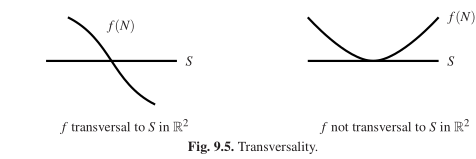
\includegraphics[scale=1]{Tu_9.5.png} 
\item \textbf{The transversality theorem}

A $C^\infty$ map $f: N \to M$ is said to be \textit{transversal} to a submanifold $S \subset M$ (Figure 9.5) if for every $p\in f^{-1}(S)$.
\begin{align*}
	f_*(T_pN)+T_{f(p)}S=T_{f(p)}M.
\end{align*}(If $A$ and $B$ are subspaces of a vector space, their sum $A+B$ is the subspace consisting all $a+b$ with $a \in A$ and $b \in B$.  Teh sum need not be a diret sum.)  The goal of this exercise is to prove that the \textit{transversality theorem:} if a $C^\infty$ map $f:n \to M$ is transveral to a regular submanifold $S$ of codeimension $k$ in $M$, then $f^{-1}(S)$ is a regular submanifold of codimension $k$ in $N$.

When $S$ consists of a single point $c$, transversality of $f$ to $S$ simply means that $f^{-1}(c)$ is a regular level set.  Thus the transversality theorem is a generalization of the regular level set theorem.  It is especially useful in giving conditions under which the intersection of two submanifolds is a submanifold.

Let $p \in f^{-1}(S)$ and $(Y,x^1,\dots,x^m)$ be an adapted chart centered at $f(p)$ for $M$ relative to $S$ such that $U\cap S=Z(x^{m-l+1}, \dots, x^m)$, the zero set of the functions $x^{_m-k+1},\dots,x^m$.  Define $g:U \to \R^k$ to be the map
\begin{align*}
	g = (x^{_m-k+1},\dots,x^m).
\end{align*}

\begin{enumerate}[label=(\alph*)]

	\item Show that $f^{-1}(U)\cap f^{-1}(S)=g\circ f^{-1}(0)$.
	\item Show that $f^{-1}(U)\cap =^{-1}(S)$ is a regular level set of teh function $g\circ f:f^{-1}(U) \to \R^k$.
	\item Prove the transverality theorem.

\end{enumerate}

\end{enumerate}
\end{document}
